\newcommand{\totalMass}{M}                        % Massa totale
\newcommand{\starMass}{m}                         % Massa singola stella
\newcommand{\numberOfStars}{N}                    % Numero di stelle
\newcommand{\radialDistance}{r}                   % Distanza radiale
\newcommand{\clusterRadius}{A}                    % Parametro di scala di Plummer 
\newcommand{\densityRho}{\rho}                    % Densità di massa
\newcommand{\potentialPhi}{\Phi}                  % Potenziale gravitazionale
\newcommand{\gravitationalConstant}{G}            % Costante gravitazionale
\newcommand{\escapeVelocity}{v_{\mathrm{esc}}}    % Velocità di fuga
\newcommand{\velV}{v}                             % Velocità
\newcommand{\totalCineticEnergy}{K}            	  % Energia Cinetica Totale
\newcommand{\totalPotentialEnergy}{U}             % Energia Potenziale Totale
\newcommand{\virialRatio}{Q}                      % Viriale
\newcommand{\semiMajorAxis}{a}                    % Semiasse Maggiore
\newcommand{\orbitEccentricity}{e}                % Eccentricità
\newcommand{\galaxyMass}{M_{\mathrm{gal}}}        % Massa galattica
\newcommand{\galaxyRadius}{A_{\mathrm{gal}}}    % Parametro di scala di Plummer 
\newcommand{\galaxyParameter}{b_{\mathrm{gal}}}   % Parametro potenziale galattico
\newcommand{\galaxyDistance}{R}                   % Distanza centro galattico
\newcommand{\velocityRescalingFactor}{\lambda}    % Fattore di riscalo per velocità
\newcommand{\deltat}{\Delta t}

\chapter{Il modello fisico}
\label{cha:modello-fisico}

\section{Notazione}
\label{sec:notazione}
La Tabella~\ref{tab:notazione} riassume i principali simboli utilizzati
nel capitolo.
\begin{table}[htbp]
	\centering
	\caption{Notazione utilizzata nel capitolo.}
	\label{tab:notazione}
	\begin{tabular}{ll}
		\hline
		\textbf{Simbolo} & \textbf{Significato} \\
		\hline
		$\numberOfStars$ & Numero di stelle dell'ammasso \\
		$\starMass$ & Massa di una singola stella \\
		$\totalMass$ & Massa totale dell'ammasso \\
		$\radialDistance$ & Distanza dal centro dell'ammasso \\
		$\clusterRadius$ & Parametro di scala del modello di Plummer \\
		$\mathbf{x}_i$ & Vettore posizione della stella $i$ \\
		$\mathbf{v}_i$ & Vettore velocità della stella $i$ \\
		$\gravitationalConstant$ & Costante gravitazionale \\
		$\densityRho(r)$ & Densità volumetrica di massa dell'ammasso \\
		$\potentialPhi(r)$ & Potenziale gravitazionale dell'ammasso \\
		$\galaxyMass$ & Massa del modello galattico \\
		$\galaxyRadius$ & Parametro di scala del modello di Plummer galattico \\
		$\galaxyParameter$ & Parametro di scala del potenziale galattico \\
		$\galaxyDistance$ & Distanza dal centro galattico \\
		$\semiMajorAxis$ & Semiasse maggiore dell'orbita dell'ammasso \\
		$\orbitEccentricity$ & Eccentricità dell'orbita dell'ammasso \\
		$\deltat$ & Passo temporale \\
		\hline
	\end{tabular}
\end{table}

\section{Generazione dell'ammasso stellare}
\label{sec:generazione-ammasso}
Per descrivere la distribuzione iniziale di un ammasso
stellare, si adotta il modello di Plummer,
che permette di definire la distribuzione delle posizioni
e delle velocità delle stelle nel contesto galattico.\cite{plummer1911}

\subsection{Il modello di Plummer}
\label{subsec:plummer}
Il modello di Plummer descrive un sistema
sferico autogravitante attraverso la sua distribuzione di massa.
È caratterizzato dalla massa totale $\totalMass$ e dal parametro
di scala $\clusterRadius$, che determina l'estensione della
distribuzione.\\
La densità volumetrica di massa in funzione della distanza
radiale $\radialDistance$ dal centro è \cite{plummer1911}:
\begin{equation}
	\densityRho(\radialDistance) =
	\frac{3\totalMass}{4\pi \clusterRadius^3}
	\left(1+\frac{\radialDistance^2}{\clusterRadius^2}\right)^{-5/2}
	\label{eq:plummer-density}
\end{equation}
Il potenziale gravitazionale associato alla distribuzione di
massa descritta dall'equazione~\eqref{eq:plummer-density}
si ottiene risolvendo l'equazione di Poisson
\cite{binneytremaine2008}:
\begin{equation}
	\potentialPhi(\radialDistance) =
	-\frac{\gravitationalConstant\totalMass}
	{\sqrt{\radialDistance^2+\clusterRadius^2}}
	\label{eq:plummer-potential}
\end{equation}

\subsection{Distribuzione delle posizioni}
\label{subsec:posizioni-iniziali}
Le posizioni iniziali delle stelle vengono estratte in modo da riprodurre la distribuzione spaziale descritta dal modello di Plummer. Integrando la densità definita nell'equazione~\eqref{eq:plummer-density} entro il raggio $\radialDistance$, si ottiene la frazione di massa racchiusa:
\begin{equation}
	\frac{M(\radialDistance)}{\totalMass}
	=
	\frac{\radialDistance^3}{(\radialDistance^2+\clusterRadius^2)^{3/2}}
	\label{eq:plummer-enclosed-mass}
\end{equation}
Questa quantità rappresenta la probabilità cumulativa di trovare una stella entro il raggio $\radialDistance$. Estraendo un numero casuale uniforme $u$ nell'intervallo $(0,1)$ e uguagliandolo a tale probabilità, si ricava il raggio iniziale di ciascuna stella:
\begin{equation}
	\radialDistance =
	\frac{\clusterRadius}{\sqrt{u^{-2/3}-1}}
	\label{eq:plummer-radius-sampling}
\end{equation}
Una volta determinato il raggio $r_i$, si estrae la direzione della posizione in modo isotropo. Il vettore posizione della stella $i$ in coordinate cartesiane è:
\begin{equation}
	\mathbf{x}_i =
	\begin{pmatrix}
		r_i\sin\theta_i\cos\phi_i \\
		r_i\sin\theta_i\sin\phi_i \\
		r_i\cos\theta_i
	\end{pmatrix}
	\label{eq:initial-position}
\end{equation}
dove $\phi_i$ è estratto uniformemente in $[0,2\pi)$ e $\cos\theta_i$ in $[-1,1]$, così da ottenere una distribuzione uniforme delle direzioni nello spazio.
Ripetendo il procedimento per tutte le $\numberOfStars$ stelle, si ottiene una distribuzione tridimensionale coerente con il profilo di Plummer.
\begin{figure}[htbp]
	\centering
	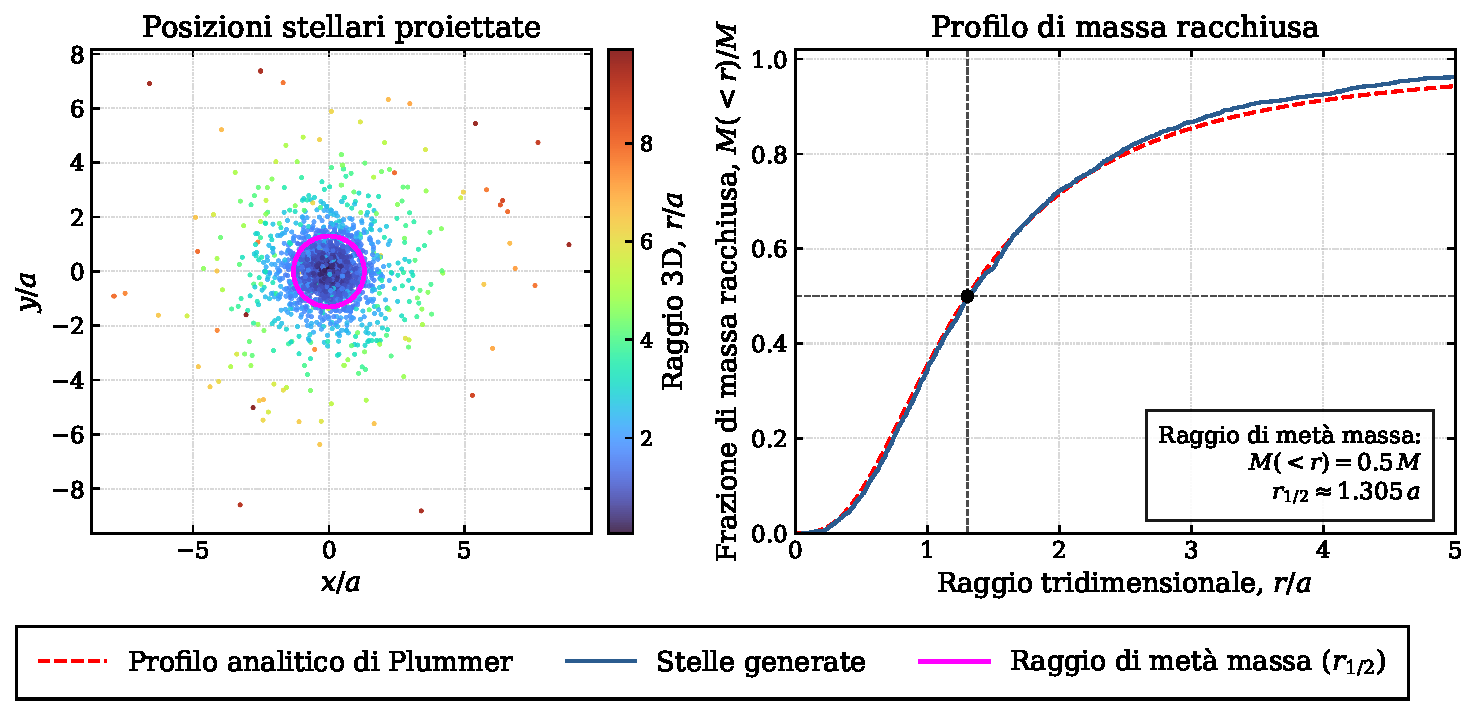
\includegraphics[width=0.8\textwidth]{./plots/initial_positions.pdf}
	\caption[Distribuzione spaziale iniziale del cluster]{Distribuzione tridimensionale delle posizioni iniziali delle stelle generate secondo il modello di Plummer ($N = 20000$, $\clusterRadius = 1.0$).}
	\label{fig:initial-positions}
\end{figure}

\subsection{Distribuzione delle velocità}
\label{subsec:velocita-iniziali}
Alle posizioni iniziali vengono associate velocità coerenti con il modello dinamico dell'ammasso. Assumendo che il potenziale gravitazionale sia nullo all'infinito, la velocità di fuga è definita come:
\begin{equation}
	\escapeVelocity(\radialDistance)
	=
	\sqrt{-2\potentialPhi(\radialDistance)}
	=
	\sqrt{\frac{2\gravitationalConstant\totalMass}
		{\sqrt{\radialDistance^2+\clusterRadius^2}}}.
	\label{eq:plummer-escape-velocity}
\end{equation}
Per il modello isotropo di Plummer, il modulo della velocità segue teoricamente la distribuzione \cite{eddington1916}:
\begin{equation}
	p(\velV \mid \radialDistance) \propto
	\velV^2
	\left(1-\frac{\velV^2}{\escapeVelocity(\radialDistance)^2}\right)^{7/2},
	\qquad
	0 \leq \velV < \escapeVelocity(\radialDistance).
	\label{eq:plummer-velocity-distribution}
\end{equation}
In alternativa al campionamento diretto di questa distribuzione, la dispersione delle velocità può essere ricavata dall'equazione di Jeans per un sistema sferico isotropo \cite{binneytremaine2008}:
\begin{equation}
	\frac{d\left[\densityRho(\radialDistance)
		\sigma_r^2(\radialDistance)\right]}{d\radialDistance}
	=
	-\densityRho(\radialDistance)
	\frac{d\potentialPhi(\radialDistance)}{d\radialDistance}.
	\label{eq:isotropic-jeans-equation}
\end{equation}
Per il modello di Plummer, la soluzione analitica è:
\begin{equation}
	\sigma_r^2(\radialDistance)
	=
	\frac{\gravitationalConstant\totalMass}
	{6\sqrt{\radialDistance^2+\clusterRadius^2}}.
	\label{eq:plummer-velocity-dispersion}
\end{equation}
In questo lavoro si utilizza la dispersione ricavata dall'equazione di Jeans per generare le componenti radiale e tangenziali della velocità mediante campionamento gaussiano. Questa scelta consente di costruire un metodo di campionamento basato sulla dispersione locale, da confrontare con il campionamento diretto della distribuzione teorica. Le particelle con energia specifica non negativa vengono scartate e le velocità sono infine riscalate per ottenere l'equilibrio viriale iniziale, come descritto nella Sezione~\ref{subsec:riscalamento-velocita}.

\begin{figure}[htbp]
	\centering
	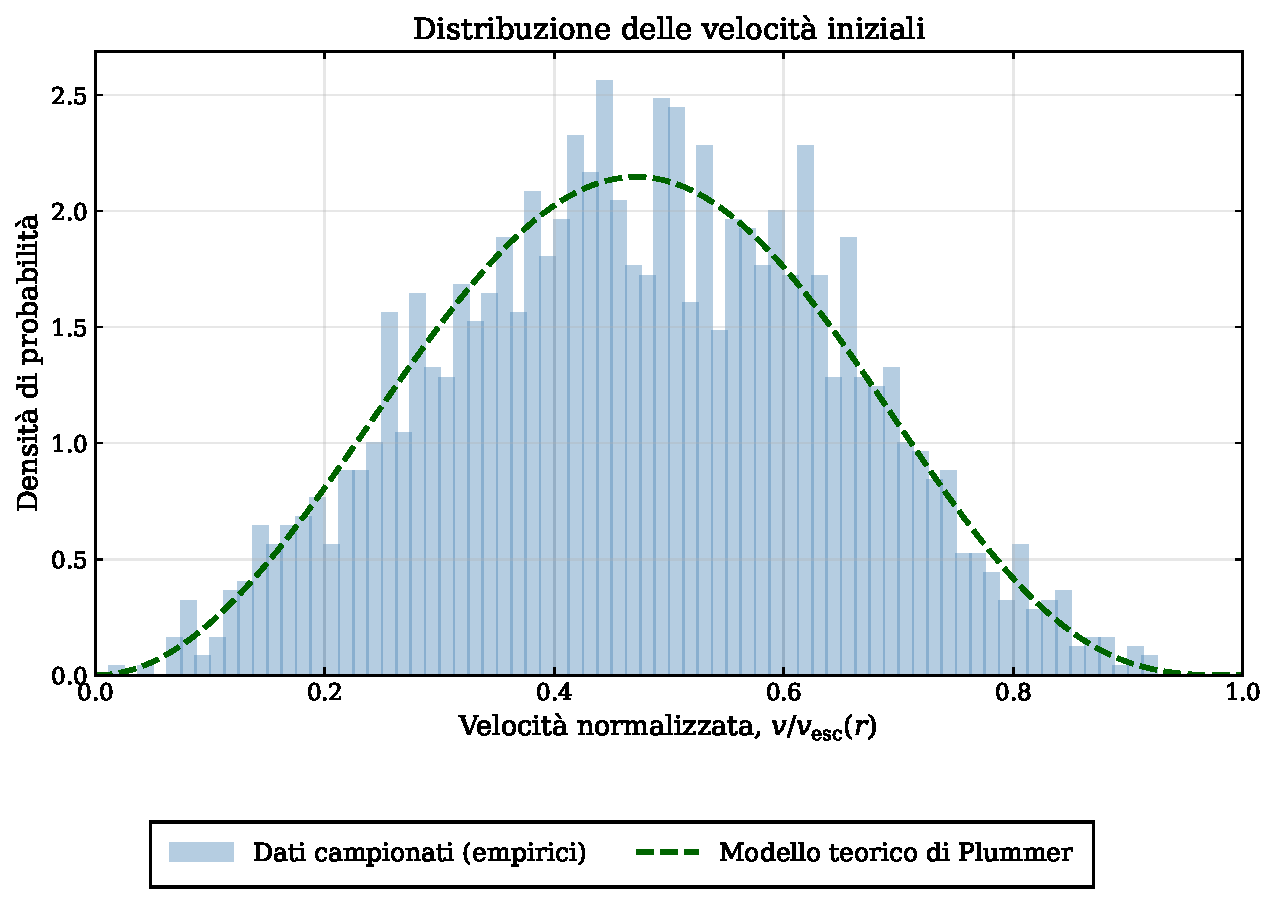
\includegraphics[width=0.6\textwidth]{./plots/velocity_distribution_comparison.pdf}
	\caption[Confronto tra le distribuzioni delle velocità iniziali]{Distribuzioni delle velocità normalizzate rispetto alla velocità locale di fuga\\($\numberOfStars = 20000$, $\clusterRadius = 1.0$).}
	\label{fig:velocity-distribution-comparison}
\end{figure}

\subsection{Condizione di equilibrio viriale}
\label{subsec:equilibrio-viriale}
Per valutare l'equilibrio dinamico iniziale dell'ammasso si considerano l'energia cinetica totale $\totalCineticEnergy$ e l'energia potenziale gravitazionale $\totalPotentialEnergy$ \cite{binneytremaine2008}. L'energia cinetica è data dalla somma dei contributi di tutte le stelle \cite{ciotti2021}:
\begin{equation}
	\totalCineticEnergy =
	\sum_{i=1}^{N} \frac{1}{2} m_i |\velV_i|^2,
	\label{eq:total-kinetic-energy}
\end{equation}
mentre l'energia potenziale gravitazionale è ottenuta sommando le interazioni tra tutte le coppie di stelle \cite{ciotti2021}:
\begin{equation}
	\totalPotentialEnergy =
	-\sum_{i=1}^{N-1}\sum_{j=i+1}^{N}
	\frac{\gravitationalConstant m_i m_j}
	{|\mathbf{x}_i-\mathbf{x}_j|}.
	\label{eq:total-potential-energy}
\end{equation}
Per un sistema autogravitante in equilibrio viriale, le due energie soddisfano la relazione \cite{ciotti2021}:
\begin{equation}
	2\totalCineticEnergy + \totalPotentialEnergy = 0.
	\label{eq:virial-equilibrium}
\end{equation}
Il rapporto viriale permette di quantificare lo scostamento da questa condizione:
\begin{equation}
	\virialRatio =
	\frac{2\totalCineticEnergy}
	{|\totalPotentialEnergy|}.
	\label{eq:virial-ratio}
\end{equation}
Il valore $\virialRatio=1$ corrisponde alla condizione viriale. Quando il rapporto calcolato dalle condizioni iniziali differisce da uno, è possibile correggerlo riscalando uniformemente le velocità, senza modificare le posizioni delle stelle.

\subsection{Riscalamento delle velocità}
\label{subsec:riscalamento-velocita}
Il campionamento delle velocità non garantisce che il rapporto viriale iniziale sia unitario. Per correggere questo scostamento, tutte le velocità vengono moltiplicate per un fattore comune $\velocityRescalingFactor$. L'energia cinetica risultante è:
\begin{equation}
	\totalCineticEnergy' =
	\velocityRescalingFactor^2 \totalCineticEnergy.
	\label{eq:rescaled-kinetic-energy}
\end{equation}
Poiché le posizioni rimangono invariate, anche l'energia potenziale resta costante durante questa operazione. Il rapporto viriale dopo il riscalamento è quindi:
\begin{equation}
	\virialRatio' =
	\velocityRescalingFactor^2 \virialRatio.
	\label{eq:rescaled-virial-ratio}
\end{equation}
Imponendo $\virialRatio'=1$, si ricava il fattore di riscalamento:
\begin{equation}
	\velocityRescalingFactor =
	\sqrt{\frac{|\totalPotentialEnergy|}
		{2\totalCineticEnergy}}
	=
	\frac{1}{\sqrt{\virialRatio}}.
	\label{eq:velocity-rescaling-factor}
\end{equation}
Il fattore viene calcolato a partire dalle energie del sistema e applicato a tutte le velocità. In questo modo si impone il rapporto viriale unitario per la configurazione iniziale, senza alterarne la distribuzione spaziale. Questa correzione riguarda il bilancio energetico globale e non garantisce, da sola, che la distribuzione delle velocità coincida con quella teorica del modello di Plummer.

\begin{figure}[htbp]
	\centering
	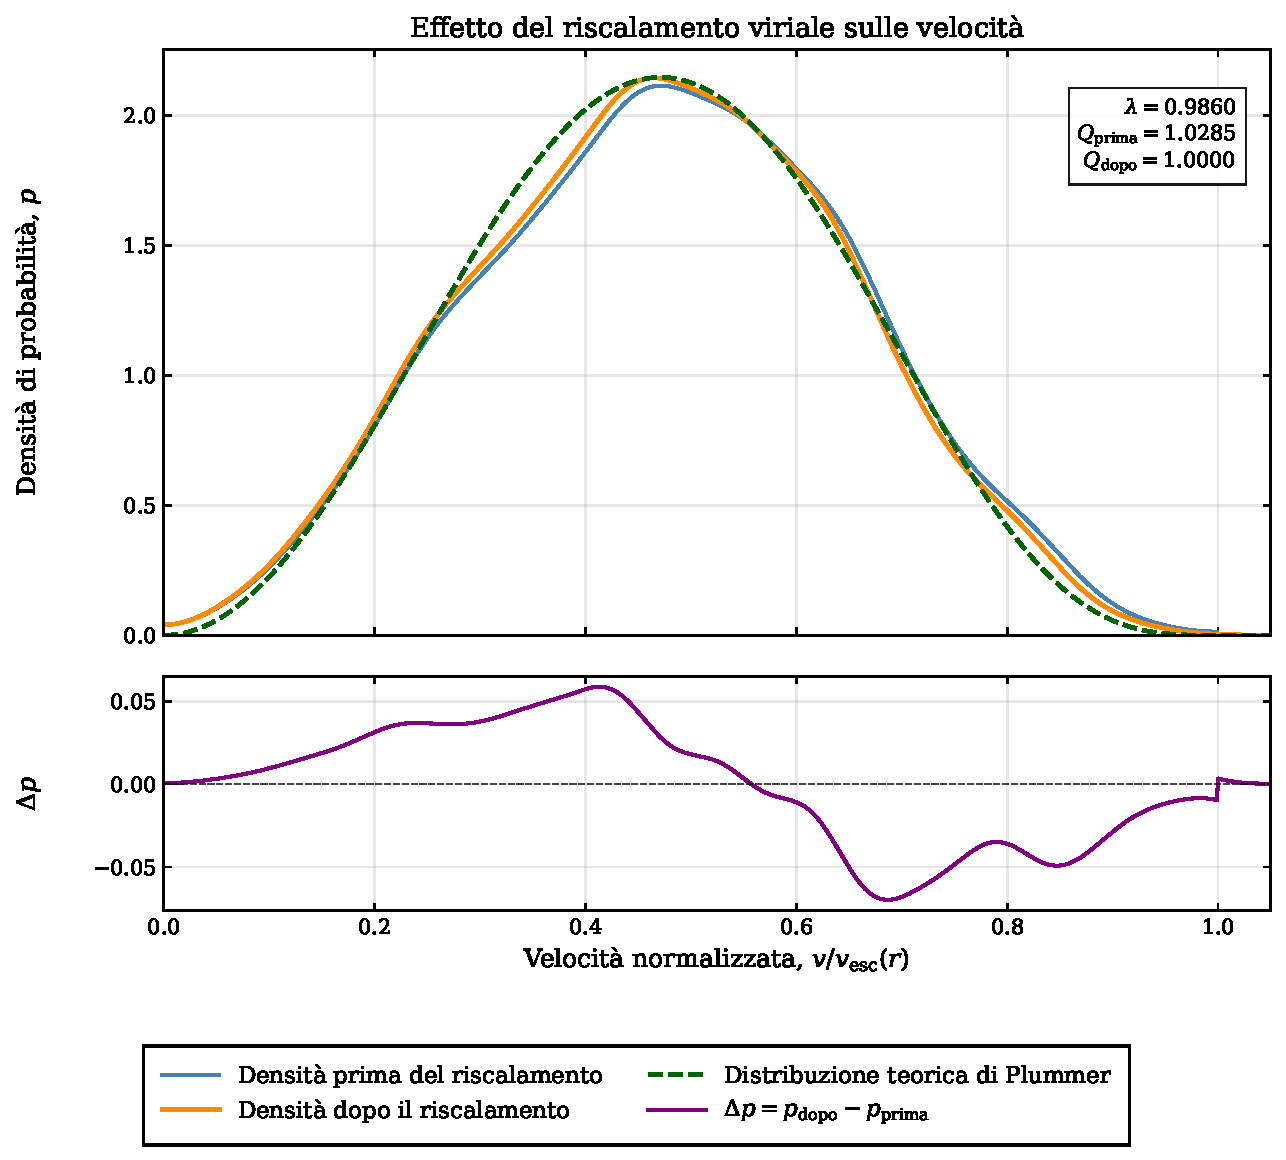
\includegraphics[width=0.6\textwidth]{./plots/velocity_rescaling.pdf}
	\caption[Confronto tra le distribuzioni delle velocità e diagnostica del viriale]{Confronto tra le distribuzioni delle velocità normalizzate ($\numberOfStars = 20000$, $\clusterRadius = 1.0$).}
	\label{fig:velocity-rescaling}
\end{figure}
\section{Evoluzione e dinamica orbitale}
\label{sec:evoluzione-ammasso}
L'evoluzione dell'ammasso stellare è descritta attraverso l'interazione gravitazionale tra le stelle e il potenziale galattico esterno, che ne determina la dinamica orbitale e l'evoluzione nel tempo.
\subsection{Potenziale galattico di Plummer}
\label{subsec:plummer-galattico}
Il potenziale gravitazionale adottato è quello di Plummer
\cite{plummer1911}, espresso in funzione della distanza $\galaxyDistance$
dal centro della galassia:
\begin{equation}
	\potentialPhi_{\mathrm{gal}}(\galaxyDistance) =
	-\frac{\gravitationalConstant \galaxyMass}
	{\sqrt{\galaxyDistance^2+\galaxyParameter^2}}
	\label{eq:galactic-plummer-potential}
\end{equation}
La forma adottata evita la singolarità del potenziale al centro,
presente nel caso di una massa puntiforme.\\
A partire dal potenziale definito nell'equazione~\eqref{eq:galactic-plummer-potential}, l'accelerazione gravitazionale esercitata dalla galassia si ottiene calcolando il gradiente del potenziale con segno opposto:
\begin{equation}
	\mathbf{a}_{\mathrm{gal}}(\mathbf{R}) =
	-\frac{\gravitationalConstant \galaxyMass}
	{(\galaxyDistance^2+\galaxyParameter^2)^{3/2}}\mathbf{R}
	\label{eq:galactic-plummer-acceleration}
\end{equation}
\begin{figure}[htbp]
	\centering
	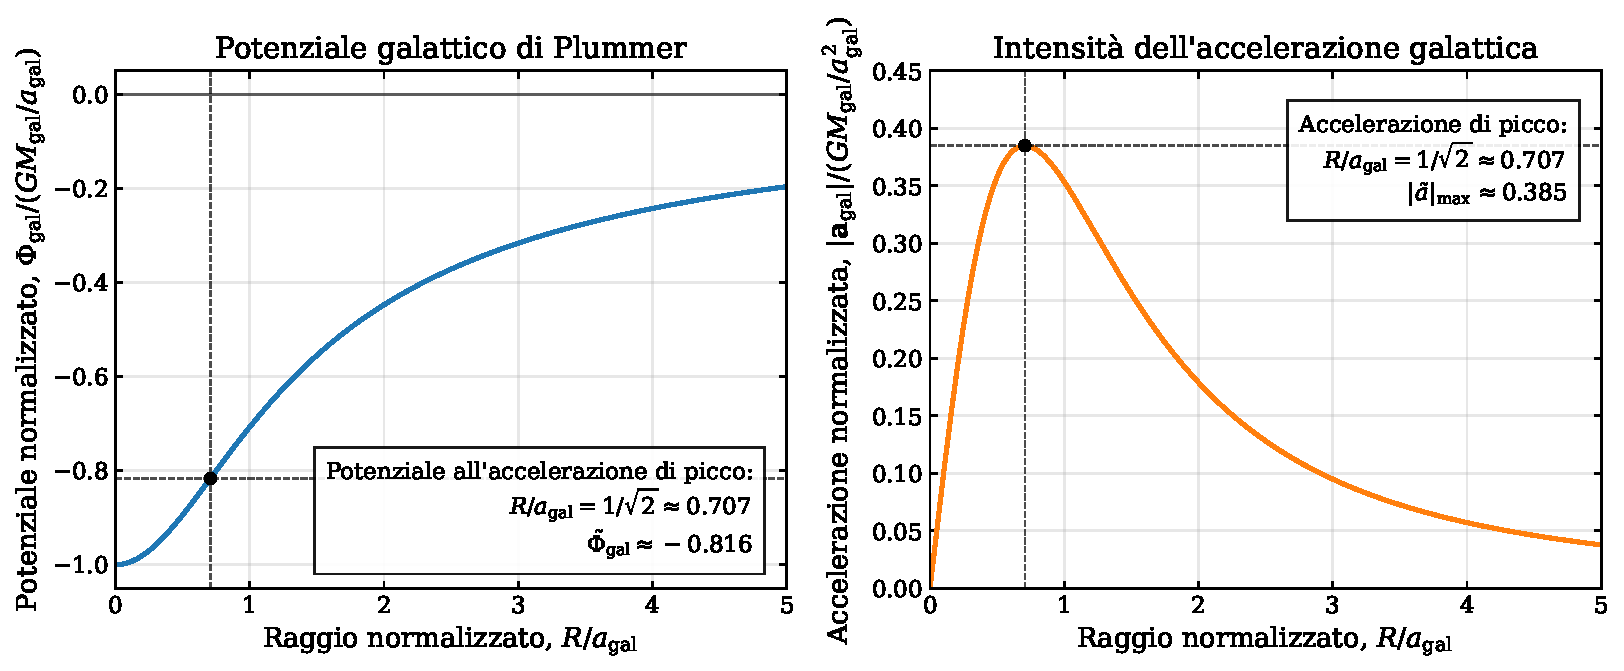
\includegraphics[width=\textwidth]{plots/galactic_plummer_potential.pdf}
	\caption{Potenziale gravitazionale e modulo dell'accelerazione del modello galattico di Plummer.}
	\label{fig:galactic-plummer}
\end{figure}

\subsection{Parametri orbitali}
\label{subsec:parametri-orbitali}
L'orbita iniziale dell'ammasso stellare viene definita attraverso il semiasse maggiore $\semiMajorAxis$ e l'eccentricità $\orbitEccentricity$. Nel caso kepleriano, questi parametri determinano le distanze di apocentro e pericentro secondo le relazioni:
\begin{equation}
	R_{\mathrm{apo}} = \semiMajorAxis(1+\orbitEccentricity),
	\qquad
	R_{\mathrm{peri}} = \semiMajorAxis(1-\orbitEccentricity)
	\label{eq:orbital-extrema}
\end{equation}
Nel modello adottato, tuttavia, il potenziale galattico è descritto dal modello di Plummer, che differisce dal potenziale kepleriano. Di conseguenza, le relazioni precedenti vengono utilizzate come scelta implementativa per determinare le distanze apsidali desiderate, senza assumere che la traiettoria risultante sia un'ellisse kepleriana.
Una volta determinate queste distanze, l'ammasso viene inizialmente collocato all'apocentro, dove la velocità è perpendicolare alla direzione radiale. Il suo modulo viene calcolato imponendo che apocentro e pericentro appartengano alla stessa orbita nel potenziale galattico adottato.
A questo scopo, si utilizzano la conservazione dell'energia meccanica specifica e del momento angolare specifico:\cite{goldstein2002}
\begin{equation}
	E = \frac{\velV^2}{2} + \potentialPhi_{\mathrm{gal}}(\radialDistance),
	\qquad
	L = \radialDistance v_{\mathrm{t}}
	\label{eq:orbital-conservation}
\end{equation}
dove $\velV$ è il modulo della velocità, $v_{\mathrm{t}}$ la sua componente tangenziale e $L$ il momento angolare specifico. In corrispondenza dell'apocentro e del pericentro, la velocità è interamente tangenziale. Uguagliando l'energia nei due punti e utilizzando la conservazione del momento angolare, si ottiene:
\begin{equation}
	L^2 =
	\frac{2\left[
		\potentialPhi_{\mathrm{gal}}(R_{\mathrm{apo}})
		-\potentialPhi_{\mathrm{gal}}(R_{\mathrm{peri}})
		\right]}
	{R_{\mathrm{peri}}^{-2}-R_{\mathrm{apo}}^{-2}}
	\label{eq:orbital-angular-momentum}
\end{equation}
Il modulo della velocità iniziale all'apocentro si ricava quindi da:
\begin{equation}
	v_{\mathrm{apo}} = \frac{L}{R_{\mathrm{apo}}}
	\label{eq:orbital-apocenter-velocity}
\end{equation}
Poiché l'approssimazione kepleriana risulta incoerente con un potenziale galattico esteso, la velocità iniziale viene ricavata rigorosamente dal potenziale di Plummer e dalle distanze apsidali, preservando la coerenza energetica del sistema. L'effetto di questa scelta è visibile in Figura~\ref{fig:orbital-methods-comparison}.
\begin{figure}[htbp]
	\centering
	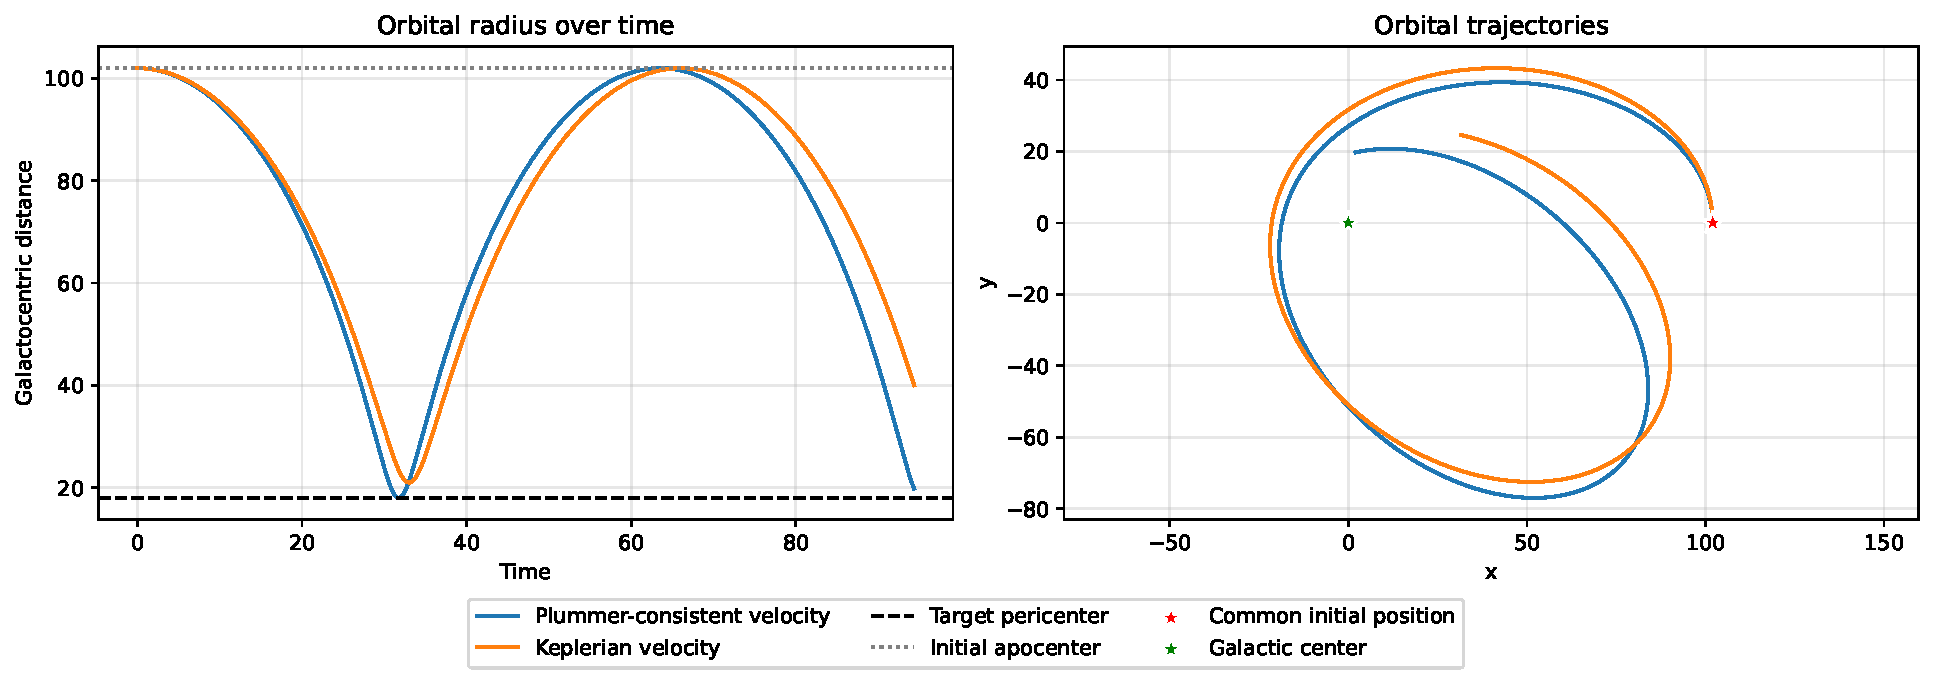
\includegraphics[width=\textwidth]{./plots/orbital_methods_comparison.pdf}
	\caption[Confronto tra i metodi di calcolo della velocità orbitale]{Confronto tra le due orbite fino al $50\%$ di divergenza del semiasse maggiore.\\($\galaxyMass = 2000.0$, $\galaxyRadius = 10.0$, $\gravitationalConstant = 1.0$, $\semiMajorAxis = 60.0$, $\orbitEccentricity = 0.7$, $\Delta t = 0.001$, Leapfrog).}
	\label{fig:orbital-methods-comparison}
\end{figure}

\subsection{Equazioni del moto}
\label{subsec:equazioni-moto}
L'evoluzione dell'ammasso stellare è descritta dalle equazioni di Newton per un sistema di particelle gravitazionalmente interagenti. Indicando con $\mathbf{x}_i$ la posizione della stella $i$ e con $m_i$ la sua massa, le equazioni del moto sono:
\begin{equation}
	\frac{d\mathbf{x}_i}{dt} = \mathbf{v}_i,
	\qquad
	\frac{d\mathbf{v}_i}{dt} = \mathbf{a}_i
	\label{eq:equations-of-motion}
\end{equation}
L'accelerazione di ciascuna stella riceve due contributi: l'interazione gravitazionale con le altre stelle dell'ammasso e il campo esterno generato dalla galassia. Nel caso newtoniano, il contributo interno è espresso da:
\begin{equation}
	\mathbf{a}_{i,\mathrm{int}} =
	-G\sum_{\substack{j=1\\j\neq i}}^N
	m_j
	\frac{\mathbf{x}_i-\mathbf{x}_j}
	{|\mathbf{x}_i-\mathbf{x}_j|^3}
	\label{eq:internal-gravitational-acceleration}
\end{equation}
L'accelerazione totale è quindi la somma del contributo interno e di quello galattico definito nella Sezione~\ref{subsec:plummer-galattico}:
\begin{equation}
	\mathbf{a}_i =
	\mathbf{a}_{i,\mathrm{int}} +
	\mathbf{a}_{\mathrm{gal}}(\mathbf{x}_i)
	\label{eq:total-acceleration}
\end{equation}
Questa formulazione permette di descrivere simultaneamente la dinamica interna dell'ammasso e la sua risposta al campo gravitazionale esterno. Le interazioni reciproche determinano l'evoluzione della struttura stellare, mentre il potenziale galattico influenza il moto complessivo dell'ammasso e può favorire la perdita di stelle gravitazionalmente non più legate alla sua componente interna \cite{binneytremaine2008}.

\subsection{Integrazione numerica}
\label{subsec:integrazione-numerica}
L'evoluzione gravitazionale di un ammasso composto da migliaia di stelle richiede l'integrazione numerica delle equazioni del moto. Per individuare un compromesso tra accuratezza e costo computazionale, sono stati confrontati diversi metodi di integrazione, con particolare attenzione allo schema \emph{leapfrog} e all'integratore adattivo IAS15 \cite{hairer2006geometric,rein2015ias15}.
Il metodo leapfrog, nella formulazione \emph{kick-drift-kick}, è un integratore simplettico del secondo ordine, adatto alle simulazioni dinamiche a lungo termine\cite{quinn1997timestepping}.\\
Indicando con $\deltat$ il passo temporale, l'aggiornamento delle posizioni e delle velocità è descritto da:\\
\begin{align}
	\mathbf{v}_{i}^{n+1/2}
	&= \mathbf{v}_{i}^{n}
	+ \frac{\deltat}{2}\mathbf{a}_{i}^{n}\\
	\mathbf{x}_{i}^{n+1}
	&= \mathbf{x}_{i}^{n}
	+ \deltat\,\mathbf{v}_{i}^{n+1/2}\\
	\mathbf{v}_{i}^{n+1}
	&= \mathbf{v}_{i}^{n+1/2}
	+ \frac{\deltat}{2}\mathbf{a}_{i}^{n+1}
	\label{eq:leapfrog-update}
\end{align}
Le prestazioni dei diversi metodi e dei passi temporali $\deltat=0.01$ e $\deltat=0.001$ vengono valutate attraverso l'errore relativo dell'energia totale, utilizzando IAS15 come riferimento ad alta precisione. Il confronto consente di quantificare l'errore introdotto dall'integrazione e di individuare il passo temporale più adeguato alle simulazioni successive.
METTERE GRAFICO QUI CONFRONTO ERRORI TRA LEAPFROG E IAS15

\subsection{Centro di massa percentile}
\label{subsec:com-percentile}
Il centro di massa globale può essere influenzato dalle stelle periferiche, soprattutto durante lo stripping mareale. Per ottenere una stima più rappresentativa della regione centrale dell'ammasso, viene introdotto un metodo basato su selezioni percentilari successive, riconducibile ai principi delle stime robuste \cite{wilcox2023guide}.
A partire dal centro di massa globale $\mathbf{x}_{\mathrm{COM}}^{(0)}$, si calcolano le distanze delle singole stelle:
\begin{equation}
	d_i^{(k)} = \left|\mathbf{x}_i-\mathbf{x}_{\mathrm{COM}}^{(k)}\right|
	\label{eq:com-percentile-distance}
\end{equation}
A ogni passaggio si mantiene la frazione più centrale del campione, ricalcolando il centro come media pesata sulle masse:
\begin{equation}
	\mathbf{x}_{\mathrm{COM}}^{(k+1)} =
	\frac{\displaystyle\sum_{i\in S_q^{(k)}}m_i\mathbf{x}_i}
	{\displaystyle\sum_{i\in S_q^{(k)}}m_i}
	\label{eq:com-percentile}
\end{equation}
La selezione utilizza in successione i percentili $80$, $65$, $50$, $35$ e $20$, interrompendosi quando rimangono meno di cinque stelle. La stessa procedura, applicata alle velocità, consente di stimare il moto del centro. La coordinata $y$ del centro percentile viene infine utilizzata per contare le orbite completate, identificando gli attraversamenti di $y=0$ dal semipiano negativo a quello non negativo.\\
Gli effetti di questa correzione sono visibili in Figura~\ref{fig:com-trajectories}, dove, già dopo una prima orbita, le due stime mostrano una divergenza attribuibile all'influenza delle stelle periferiche sul centro di massa globale.
\begin{figure}[htbp]
	\centering
	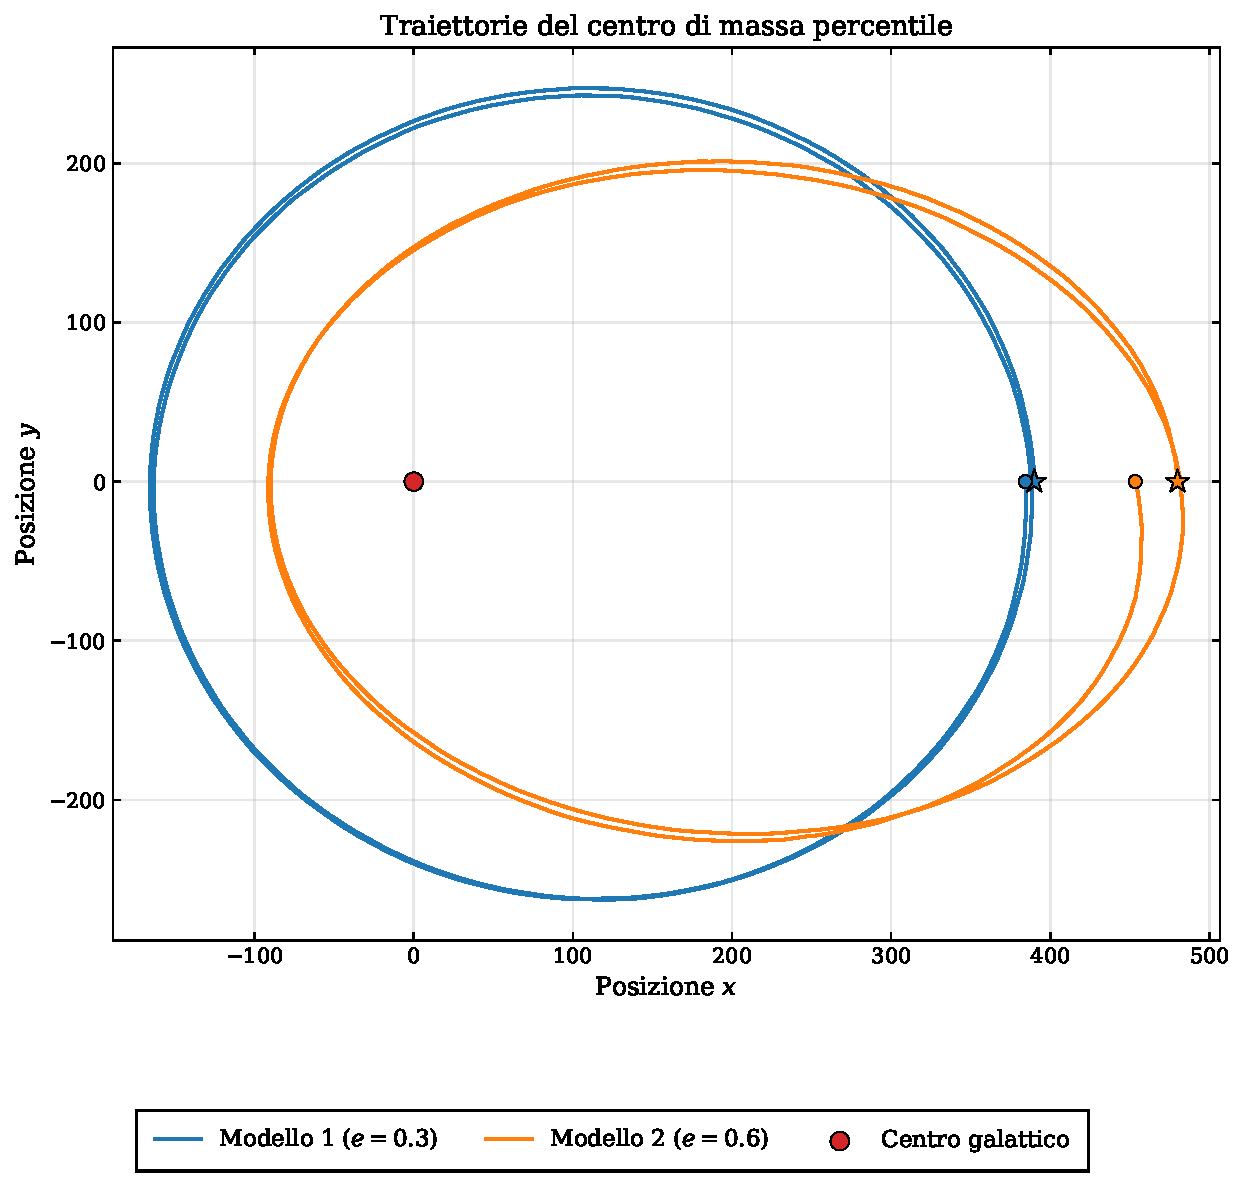
\includegraphics[width=\textwidth]{./plots/com_trajectories.pdf}
	\caption[Traiettorie del centro di massa classico e percentile]{Traiettorie di due orbite del centro di massa classico e percentile.\\($\numberOfStars = 2000$, $\clusterRadius = 1.0$, $\galaxyMass = 2000.0$, $\galaxyRadius = 10.0$, $\gravitationalConstant = 1.0$, $\semiMajorAxis = 294.0$, $\orbitEccentricity = 0.7$, $\deltat = 0.001$, Leapfrog)}
	\label{fig:com-trajectories}
\end{figure}
